\documentclass{beamer}

\usetheme{CambridgeUS}
\usepackage{animate}

\usepackage[utf8x,utf8]{inputenc} % make weird characters work
\usepackage[serbian]{babel}

\usepackage{graphicx}
\graphicspath{{Figures/}{./}} % Specifies where to look for included images
\usepackage{color}

\usepackage{mathpazo} % Use the Palatino font by default
\usepackage{amsmath}


\usepackage{verbatim}

% -------------------------------------------------

% definišemo korisne komande
\newcommand{\en}[1]{(engl. \textit{#1})}
\newcommand{\lat}[1]{(latin. \textit{#1})}
\newcommand{\keyword}[1]{\textbf{#1}}
\newcommand{\ikeyword}[1]{\textit{\textbf{#1}}}
\newcommand{\tabhead}[1]{\textbf{#1}}
\newcommand{\code}[1]{\texttt{#1}}
\newcommand{\file}[1]{\texttt{\bfseries#1}}
\newcommand{\option}[1]{\texttt{\itshape#1}}


\newcommand{\uniprot}{\textit{UniProt} }
\newcommand{\uniprotkb}{\textit{UniProtKB} }
\newcommand{\swissprot}{\textit{Swiss-Prot} }
\newcommand{\trembl}{\textit{TrEMBL} }

\newcommand{\kw}[1]{\textbf{\textit{KW: #1}}}
\newcommand{\mf}[1]{\textbf{\textit{MF: #1}}}

\newtheorem{definicija}{Definicija}

% -------------------------------------------------

% \title{Bioinformatička analiza povezanosti funkcije i neuređenosti proteina}
\title[Povezanost funkcije i neuređenosti proteina]{Bioinformatička analiza povezanosti funkcije i neuređenosti proteina}
% \subtitle{Master Rad}

\author{Goran Vinterhalter}
\institute[Matematički fakultet]{ Matematički fakultet, Beogradski univerzitet }
\date{\today}

% This is only inserted into the PDF information catalog. Can be left
% out. 

% If you have a file called "university-logo-filename.xxx", where xxx
% is a graphic format that can be processed by latex or pdflatex,
% resp., then you can add a logo as follows:

% \pgfdeclareimage[height=0.5cm]{university-logo}{university-logo-filename}
% \logo{\pgfuseimage{university-logo}}


% Delete this, if you do not want the table of contents to pop up at
% the beginning of each subsection:

% \AtBeginSubsection[]
% {
%   \begin{frame}<beamer>{Outline}
%     \tableofcontents[currentsection,currentsubsection]
%   \end{frame}
% }

% Let's get started
\begin{document}

\setbeamertemplate{caption}{\raggedright\insertcaption\par}


\begin{frame}
  \titlepage
\end{frame}

% \begin{frame}{Outlin
%   \tableofcontents
%   % You might wish to add the option [pausesections]
% \end{frame}

\section{Uvod}

\begin{frame} 
  \begin{figure}
    \hspace*{-0.2cm}
    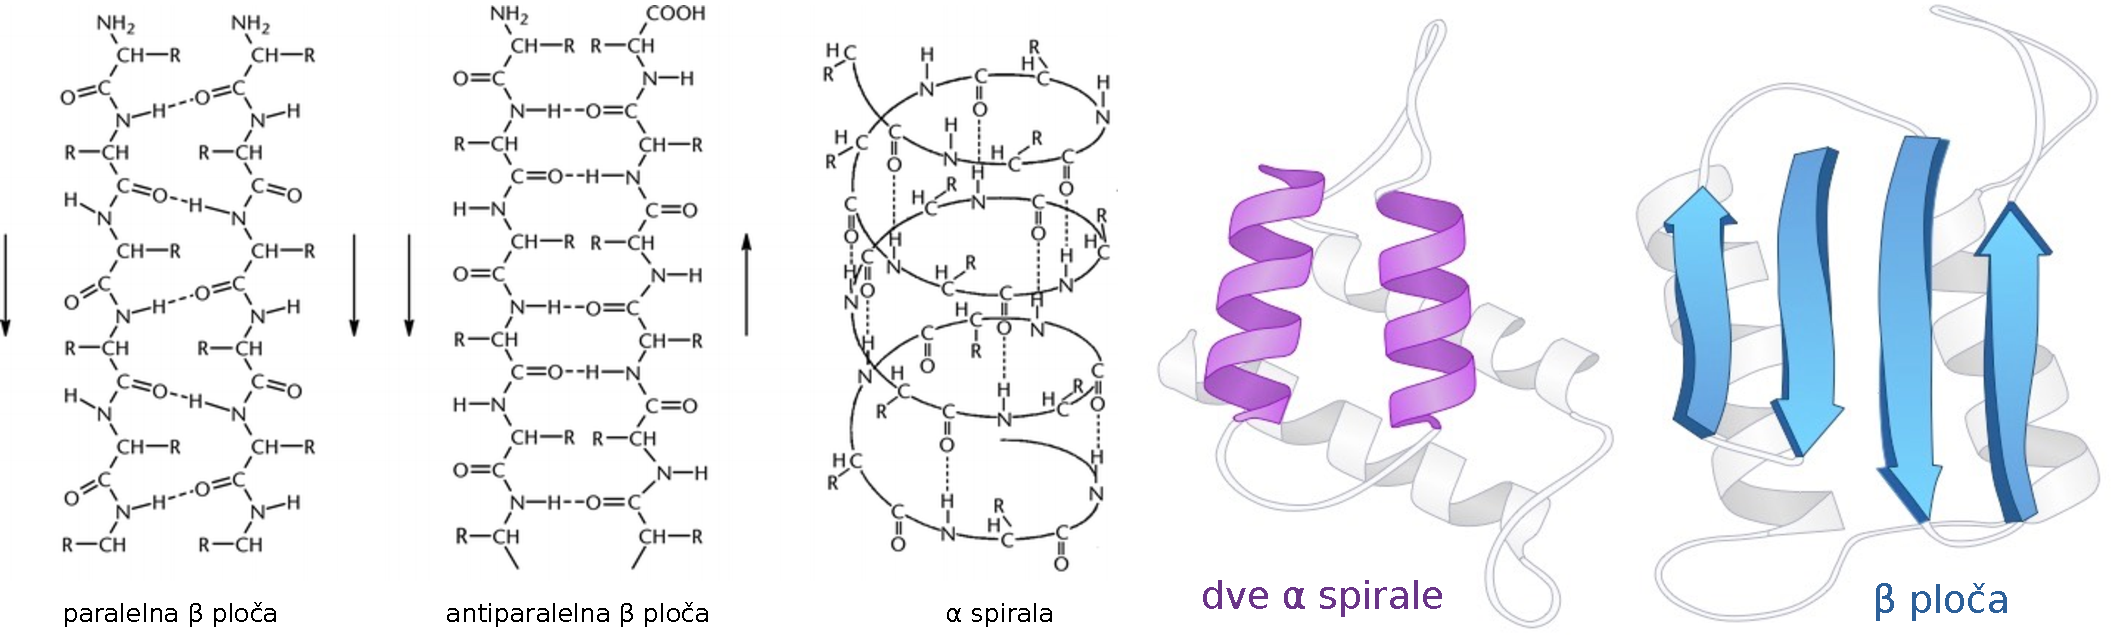
\includegraphics[scale=0.35]{uvod/sekundarna.pdf}
  \end{figure}
  \begin{figure}
    \centering
    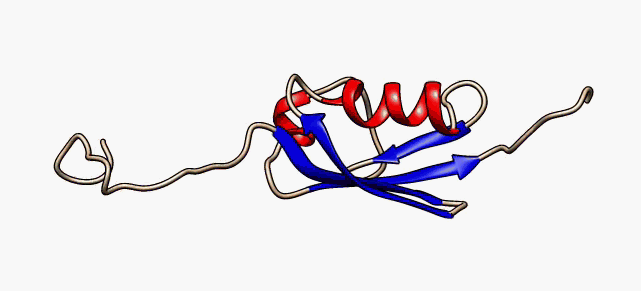
\includegraphics[scale=0.30]{sumo/sumo1-0.png}
  \end{figure}
\end{frame}

\subsection{Inherentno neuređeni proteini}
\begin{frame} {Šta su to neuređeni proteini?}

  Inherentno neuređeni protein \en{Intrinsically disordered protein, IDP}
  \begin{itemize}
    \item Funkcionalan protein
    \item Izostanak fiksne trodimenzionalne strukture, celovito ili delimično 
    \item Jedan ili više neuređenih regiona (IDPr)
  \end{itemize}

  \begin{columns}
    \column{0.5\textwidth}
    Dunker (2001):
    \begin{enumerate} \small
      \item Uređen protein 
      \item Topljiva globula\\ \en{molten globule} 
      \item Pre-topljiva globula \\\en{pre-molten globule} 
      \item Nasumično klupko \\\en{random coil} 
    \end{enumerate}

    \column{0.5\textwidth}
    Uverski (2016):
    \begin{itemize} \small
      \item foldon \en{foldon} - nezavisno organizujuća jedinica proteina
      \item indukativni foldon \\\en{inducible foldon} 
      \item ne-foldon \en{non-foldon} 
      \item polu-foldon \en{semi-foldon} 
      \item anti-foldon \en{unfoldons} 
    \end{itemize}
  \end{columns}

\end{frame}


% \begin{frame}
%   \animategraphics[autoplay,loop,width=\linewidth]{1}{sumo/sumo1-}{ }{}
% \end{frame}]


\subsection{Funkcija proteina}

\begin{frame}{Ontologija gena}

  \begin{columns}
    \column{0.4\textwidth}

    Prostori imena:
    \begin{itemize}
      \footnotesize
      \item Molekulska funkcija (MF)
      \item Ćelijske komponente  (CC)
      \item Biološki procesi (BP)
    \end{itemize}


    Molekulske funkcije:
    \begin{itemize}
      \item \textit{$x$ binding} 
      \item \textit{$<$enzyme$>$ activity} 
      \item \textit{$x$ receptor activity} 
      \item \textit{$x$ transporter activity} 
    \end{itemize}


    \column{0.8\textwidth}
    \begin{figure}[h!]
      \vspace*{-0.7cm}
      \hspace*{-3.0cm} 
      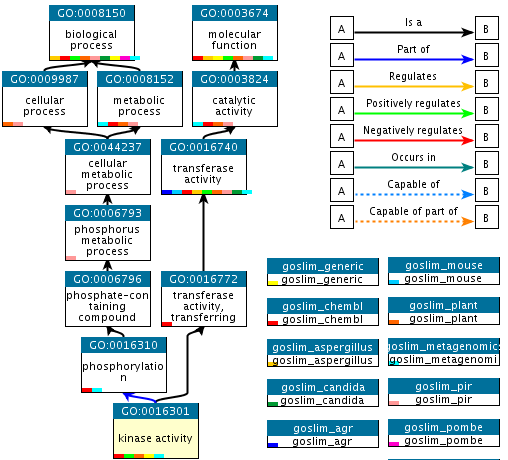
\includegraphics[width=0.8\linewidth]{img/kinase.png}
    \end{figure}

  \end{columns}
  
\end{frame}


\begin{frame}{Baza podataka \swissprot}

  \begin{columns}
    \column{0.5\textwidth}

    \begin{itemize}
      \small
      \item Podskup baze \uniprot
      \item Visoko kvalitetne sekvence, ručno proverene anotacije 
      \item minimalno redundantni unosi
      \item Funkcija anotirana \keyword{ključnim rečim} \en{keywords}
      \item Identifikacioni broj \keyword{AC} \\ \en{accession number}
        \begin{itemize}
          \item primarni
          \item sekundarni
        \end{itemize}
      \item dokaz o postojanju proteina
      \item prosečna dužina prot. je između 100 i 500AK
    \end{itemize}




    \column{0.5\textwidth}
\begin{figure}[h!]
  \centering
  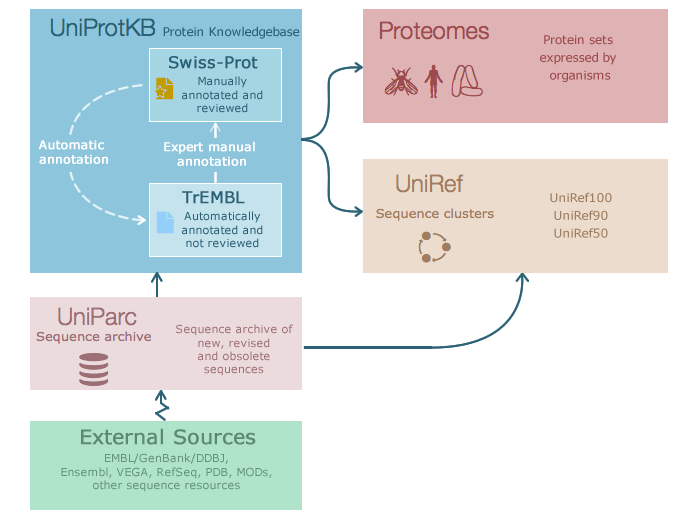
\includegraphics[width=1\linewidth]{uniprot_overview.png}
  \caption{Šematski prikaz povezanosti \uniprot}
\end{figure}

  \end{columns}
  
\end{frame}

\section{Podaci}


\begin{frame}
  \frametitle{Podaci iz referentnog rada}

  \begin{itemize}
    \item \swissprot v48 iz 2005. (oko 200 000 sekvenci)
    \item Kontrolisani vokabular, ključne Svis-Prot-reči (ključne reči) (710 kw)
    \item \swissprot sadrži statistički redundantne sekvence
    \item Klasterovanje u proteinske familije (27 217 familija)
  \end{itemize}

\end{frame}

\begin{frame}
  \frametitle{Korišćeni podaci}

  \begin{itemize}
    \item \textit{CAFA3}-skup podataka (trening skup sa \textit{CAFA3 takmičenja})
    \item \textit{CAFA3}-skup je podskup baze \swissprot
    \item GO-termini za anotaciju funkcija
    \item pretpostavljamo da sekvence iz \textit{CAFA3}-skupa nisu statistički
          redundantne
  \end{itemize}

  \begin{figure}
    \centering 
    \hspace*{-0.5cm} 
    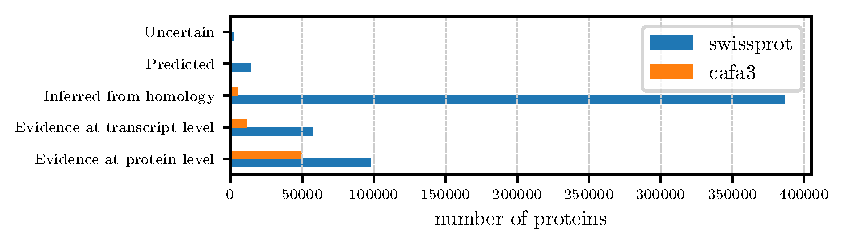
\includegraphics[scale=0.8]{plots/cafa3_pe}
    \vspace*{-0.5cm} 
    \caption{Pouzdanost postojanja proteina iz CAFA3-podskupa }
  \end{figure}
\end{frame}





% ---------------------------------------------------------------------------
\section{Metod}
% ---------------------------------------------------------------------------



\begin{frame}{Postavka}
  \begin{block}{Idealan slučaj}
    Za posmatrane proteine poznati su nam njihovi IDPr i njihov pojedinačajn
    uticaj na funkciju.    Nažalost postoje mnoga ograničenja:
    \begin{itemize}
      \item Baza \textit{\keyword{DisProt}} sadrži svega 803 proteina sa
        opisanih 2167 IDPr.  

      \item Kvalitet dobijenih karakterizacija iz baze DisProt je diskutabilan.
        

      \item Čak i konsenzus nekoliko različitih prediktora ne daje dovoljno
        pouzdane rezultate o lokaciji neuređenog regiona.
    \end{itemize}
  \end{block}

  

  \begin{block}{Jednostavna alternativa idealnom slučaju}
    Pretpotavićemo da veći udeo neuređenih u odnosu na uređene proteine podrazumeva
    da funkcija zavisi više od neuređenih regiona nego uređenih proteinskih domena. 
  \end{block}
\end{frame}


\begin{frame}{Predikcija neuređenosti proteina}
  \begin{definicija}
    \label{pdis_def}
    Protein je \keyword{putativno neuređen} \en{putatively disordered}
    (najverovatnije neuređen, u daljem tekstu \keyword{neuređen}) ako sadrži bar
    jedan region veći ili jednak od 40 uzastopnih aminokiselina takvih da im je
    predviđena neuređenost iznad 0.5. 
  \end{definicija}

  Onda definišemo operator $d$ takav da za svaku proteinsku sekvencu $s_i$ važi:
  \[   
    d(s_i) = 
    \begin{cases}
    1 & \text{ako je  $s_i$ \keyword{neuređena} (gornja Definicija) }\\
    0 & \text{suprotno}
  \end{cases}
\]
\end{frame}


\begin{frame}{$P_L$: zavisnost dužine proteina i predikcije neuređenosti}
  Neka je $S_L$ skup proteina sa dužinama iz intervala $[L-l, L+l]$ gde je
  $l = 0.1 \cdot L$.  Na primer, skup $S_{100}$ sadrži proteine iz intervala
  $[90, 110]$, a $S_{500}$ iz intervala $[450, 550]$.

  $$ S_L = \{s_i :  | L -  | s_i | | \le l  \}, \quad   |s_i| \text{ je dužina
  sekvence}  $$

  $$ P_L = \dfrac{ \sum_{s_i \in S_L} d(s_i)} {| S_L |}, \quad   |S_L| \text{
  je kardinalnost skupa}$$
\end{frame}


\begin{frame}{}
  \begin{figure}[]
    \centering
    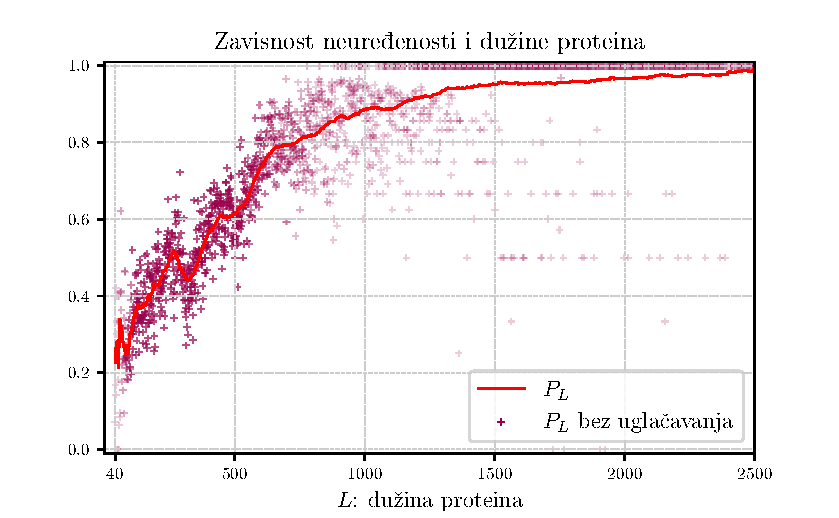
\includegraphics[scale=0.8]{plots/PL_F}
    \caption {
      \footnotesize Zavisnost neuređenosti i dužine proteina iz CAFA3-skupa
      minimalne dužine 40 AK
    }
  \end{figure}
\end{frame}

\begin{frame}{}
  \begin{itemize}
    \item $P_L random$ - slučajni model \en{random model} 
    \item $P_L uniform$  - model uniformne verovatnoće  \en{uniform model}
  \end{itemize}

  \begin{figure}[th]
    \centering
    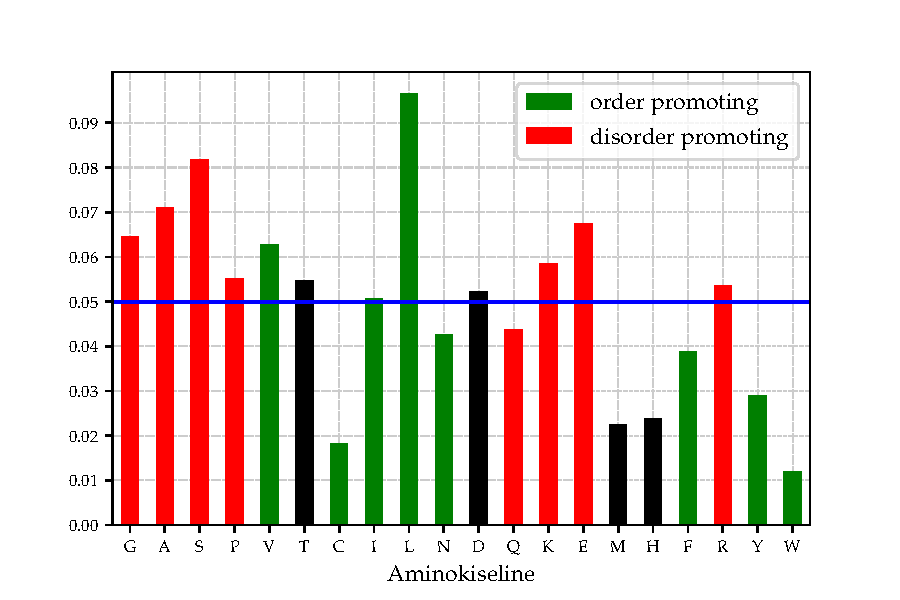
\includegraphics[scale=0.7]{plots/AK_ucestalost}
    \vspace{-0.2cm}
    \caption{ \footnotesize Učestalost aminokiselina u CAFA3-podacima }
  \end{figure}
\end{frame}

\begin{frame}
  \begin{figure}[th]
    \centering
    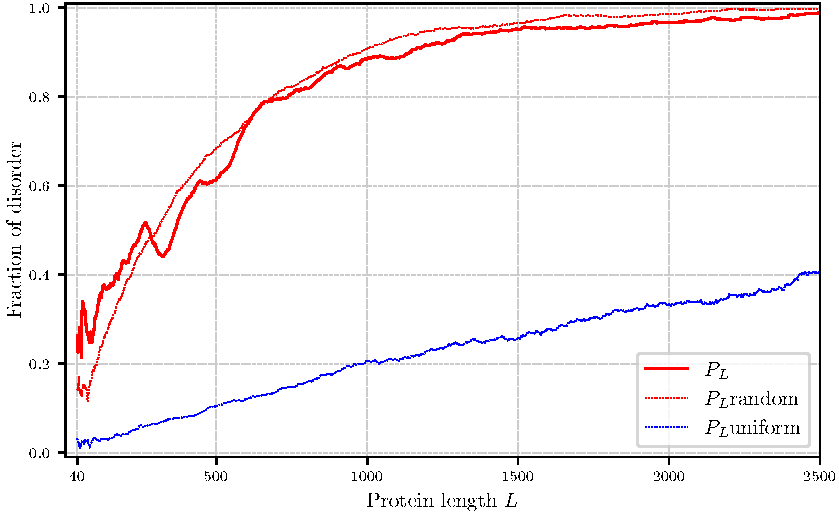
\includegraphics[scale=0.8]{plots/PL_F_cmp}
    \caption{Upoređivanje $P_L$, $P_L random$ i $P_L uniform$ modela nad
    CAFA3-podacima}
  \end{figure}
\end{frame}

% \begin{frame}
%   \begin{figure}
%     \centering
%     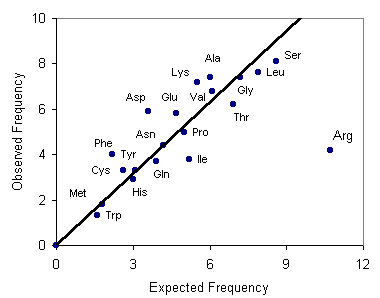
\includegraphics[scale=0.7]{aminoacid}
%     \caption{Očekivana i izmerena učestalost aminokiselina (kod kičmenjaka)}
%   \end{figure}
% \end{frame}

\begin{frame}{Ocenjivanje zavisnosti funkcije od neuređenosti}

  \begin{itemize}
    \item 
      Neka je $S_j$ skup proteina koji imaju pridruženu funkciju $j$. Tada se
      učestalost neuređenih proteina u oznaci $F_j$ može izračunati kao:
      $$F_j = \dfrac{\sum_{s_i \in S_j} d(s_i)} {|S_j|} $$

    \item
      Nultu hipotezu $Y_j$ za $F_j$  def. preko Bernulijeve slučajne prom. $X_L$
      $$
      Y_j = \dfrac {\sum_{s_i \in S_j} {X_{|s_j|}}}{|S_j|}
      \quad \quad \quad
    X_L : \begin{pmatrix} 0 & 1\\ P_L & 1-P_L \end{pmatrix}
      $$
      \begin{itemize}
        \item $p<0.05$: funkcija je povezana (korelirana) sa uređenim proteinima
        \item $p>0.95$: funkcija je povezana (korelirana) sa neuređenim proteinima
        \item suprotno: povezanost (koreliranost) funkcije $j$ nije statistički značajno  
      \end{itemize}


  \end{itemize}

\end{frame}

\begin{frame}{Ocenjivanje zavisnosti funkcije od neuređenosti}
  \begin{definicija}
    \keyword{Neuređenost} funkcije (GO-termina ili ključne reči) je mera učestalosti
    neuređenih proteina ($F_j$).
  \end{definicija}
  \begin{definicija}
    Funkcija (GO-termin ili ključna reč) je:
    \begin{itemize}
      \item \keyword{neuređena} ako je povezana ($p<0.05$) sa neuređenim proteinima
      \item \keyword{uređena} ako je povezana ($p>0.95$) sa uređenim proteinima
    \end{itemize}
  \end{definicija}
  \begin{definicija}
    \keyword{Statistički najznačajnije} uređene/neuređene funkcije
    (GO-termini ili ključne reči) su one koje imaju najmanji/najviši Z-skor.
  \end{definicija}
\end{frame}


% \begin{frame}{Ocenjivanje zavisnosti funkcije od neuređenosti}
%
% Neka je $S_j$ skup proteina koji imaju pridruženu funkciju $j$. Tada se
% učestalost neuređenih proteina u oznaci $F_j$ može izračunati kao:
% $$F_j = \dfrac{\sum_{s_i \in S_j} d(s_i)} {|S_j|} $$
%
%
% \begin{definicija}
%   \keyword{Neuređenost} funkcije (GO-termina ili ključne reči) je mera učestalosti
%   neuređenih proteina ($F_j$).
% \end{definicija}
%
%
% \end{frame}
%
% \begin{frame}{Ocenjivanje zavisnosti funkcije od neuređenosti}
%
%   Nultu hipotezu ($Y_j$) za $F_j$  definišemo preko Bernulijeve slučajne prom. $X_L$
%   $$
%   Y_j = \dfrac {\sum_{s_i \in S_j} {X_{|s_j|}}}{|S_j|}
%   \quad \quad \quad
%   X_L : \begin{pmatrix} 0 & 1\\ P_L & 1-P_L \end{pmatrix}
%   $$
%
%   \begin{itemize}
%     \item $p<0.05$: funkcija je povezana (korelirana) sa uređenim proteinima
%     \item $p>0.95$: funkcija je povezana (korelirana) sa neuređenim proteinima
%     \item suprotno: povezanost (koreliranost) funkcije $j$ nije statistički značajno  
%   \end{itemize}
%
%
%   \begin{definicija}
%     Funkcija (GO-termin ili ključna reč) je \keyword{neuređena} ako je povezana
%     ($p<0.05$) sa neuređenim proteinima, a uređena ako je povezana ($p>0.95$) sa
%     uređenim proteinima.
%   \end{definicija}
% \end{frame}
%
%
%
%
% \begin{frame}{Ocenjivanje zavisnosti funkcije od neuređenosti}
%   Referentni autori tvrde da se za veće skupove $S_j$, raspodela $Y_j$ ponaša
%   kao normalna. To znači da se ocena Z-skor može dobiti kao
%   $Z_j=(F_j-\mu_j)/\delta_j$ gde je $\mu_j$ očekivanje, a $\delta_j$ standardna
%   devijacija. Onda se Z-skor može koristiti za rangiranje (ne)uređenih funkcija
%   po statističkoj značajnosti.
%
%   \begin{definicija}
%     \keyword{Statistički najznačajnije} uređene/neuređene funkcije
%     (GO-termini ili ključne reči) su one koje imaju najmanji/najviši Z-skor.
%   \end{definicija}
%
% \end{frame}


\section{Priprema podataka}

\begin{frame}

  \begin{enumerate}
    \item Objedinjavanje baze \swissprot i njenog CAFA3-podskupa
      \begin{itemize}
        \item Dobijeno je 66 530 validnih proteina (od ukupno 66 599)
        \item Anotacije (term \& kw) su preuzete iz baze \swissprot
        \item Sekvence su zadržane originalne iz CAFA3-skupa
      \end{itemize}
    \item Grupisanje proteina po GO-terminima
      \begin{itemize}
        \item Dobijeno je 1781 MF-termin koji anotira min. 20 proteina.
              Bez grupisanja bilo bi samo 1146 MF-termina.
      \end{itemize}
    \item Preslikavanje između ključnih MF-reči i MF-termina


  \end{enumerate}

  \begin{table}
    \begin{tabular}{|r|c|c|c|c|c|}
      \hline
      & ukupno & nema pres. & pres. MF & pres. BP & pres. CC.      \\
      \hline
      ključ. MF-reči  & 195    &  20       &  104     & 54      & 11           \\
      \hline
    \end{tabular}
  \end{table}
  
\end{frame}

\begin{frame}
  \begin{figure}[!th]
    \centering
    \vspace*{-0.2cm} 
    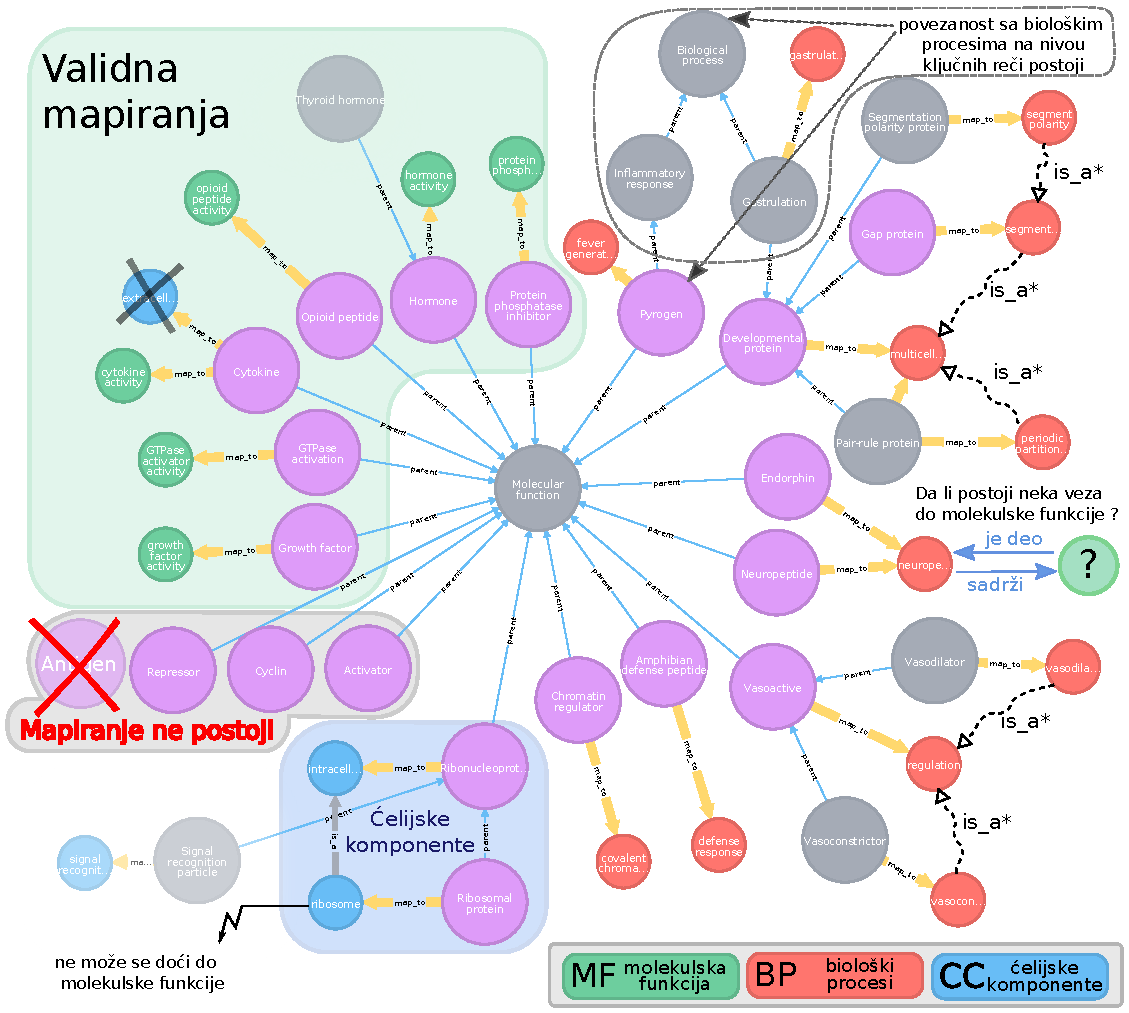
\includegraphics[scale=0.5]{Figures/plots/kw_dis2go.pdf}
  \end{figure}
\end{frame}

\begin{frame}
  \begin{figure}[!th]
    \centering
    \vspace*{-0.49cm} 
    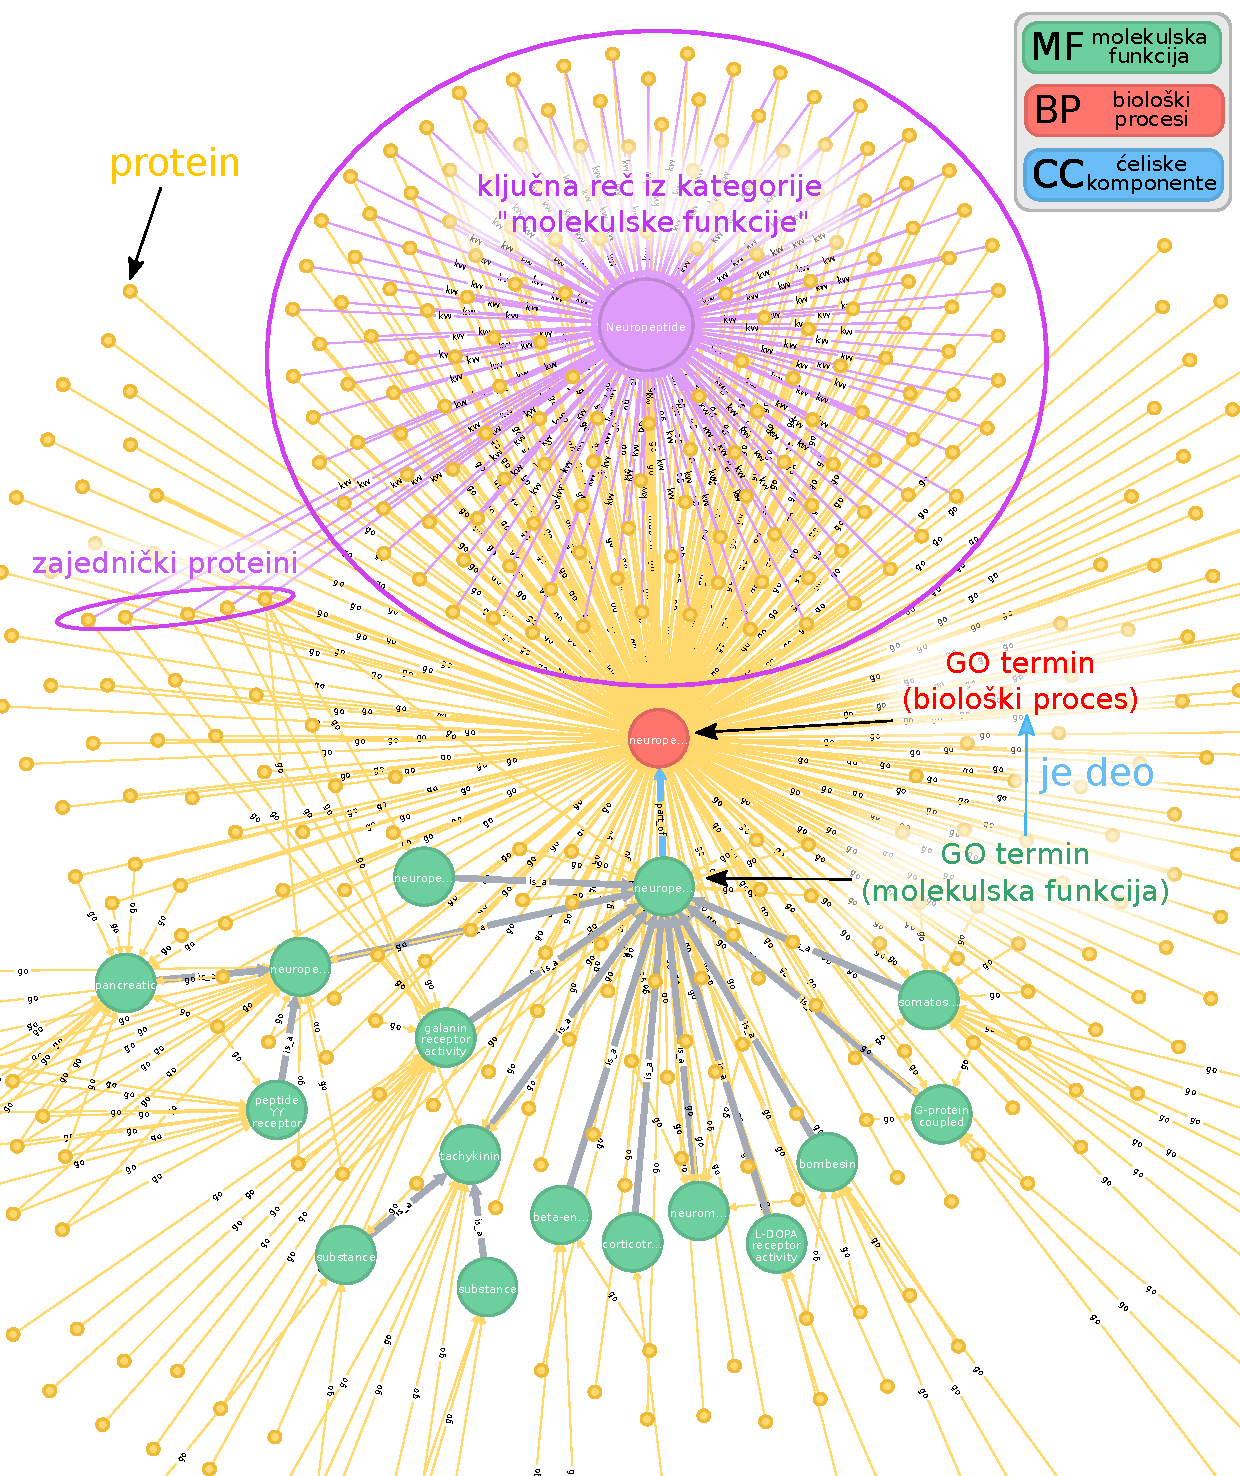
\includegraphics[scale=0.45]{Figures/plots/Neuropeptide2go.pdf}
  \end{figure}
\end{frame}


\begin{frame}{Metod sličnih anotacija}
  \begin{itemize}
    \item Žakardov indeks \en{Jaccard index}, kraće \keyword{Ji}  
$$J(A,B) = \dfrac{|A \cap B|}{|A \cup B|} =  \dfrac{|A \cap B|}{|A|+|B|-|A \cap B|}$$
$$  J(A,B) \in [0, 1] $$
\[   
  J(A,B) = 
    \begin{cases}
      1,&A=B  \\
      0,&A\cap B=\emptyset
    \end{cases}
\]

  \item  Preslikavanja su dopunjena sa 64 izvedena preslikavanja ($Ji>0.1$).

  \end{itemize}
\end{frame}


\begin{frame}

  \footnotesize
  \begin{tabular}{|p{4.2cm}|c|c|c|p{5cm}|}
    \hline
    \bf \textit{ključna MF-reč } & \bf n\_kw & \bf Ji & \bf n\_go & \bf \textit{MF-termin} \\
    \hline
    \hline
    Dermonecrotic toxin                & 148   & 0.96  & 142   & phospholipase D activity \\ \hline
    \keyword{Ribosomal protein}        & 49054 & 0.91  & 48096 & structural constituent of ribosome \\ \hline
    Complement system impairing  toxin & 160   & 0.81  & 142   & phospholipase D activity \\ \hline
    Hemagglutinin                      & 397   & 0.75  & 299   & host cell surface receptor binding \\ \hline
    Mutator protein                    & 255   & 0.75  & 288   & damaged DNA binding \\ \hline
    Antifreeze protein                 & 10    & 0.7   & 7     & ice binding \\ \hline
    Light-harvesting polypeptide       & 90    & 0.68  & 61    & bacteriochlorophyll binding \\ \hline
    Cyclin                             & 197   & 0.61  & 124   & cyclin-dependent protein ... \\ \hline
    Defensin                           & 55    & 0.55  & 32    & CCR6 chemokine receptor binding \\ \hline
    \keyword{Ribonucleoprotein}        & 50698 & 0.54  & 28317 & rRNA binding \\ \hline
    Neurotoxin                         & 2734  & 0.53  & 4145  & toxin activity \\ \hline
    Photoprotein                       & 40    & 0.48  & 19    & alkanal monooxygenase ... \\ \hline
    \keyword{Endorphin}                & 48    & 0.45  & 32    & opioid peptide activity \\ \hline
    Protein synthesis inhibitor        & 150   & 0.43  & 67    & rRNA N-glycosylase activity \\ \hline
    \keyword{Neuropeptide}             & 561   & 0.42  & 267   & neuropeptide hormone activity \\ \hline
    ... & ... & ... & ... &  ...\\
    \hline
    \keyword{Vasoactive}                            & 243   & 0.17  & 489   & hormone activity \\ \hline
    \keyword{Chromatin regulator}                   & 1939  & 0.12  & 861   & chromatin binding \\ \hline
    \keyword{Developmental protein}                 & 6285  & 0.12  & 2464  & sequence-specific DNA binding \\ \hline
  \end{tabular}

\end{frame}




\section{Rezultati}


\begin{frame}{Rezultati}

  \begin{table}[htpb]
    \centering
    \begin{tabular}{|r|c|c|c|}
      \hline
      & \small referentni rezultati   & \multicolumn{2}{c|}{ novi rezultati} \\
      & Xie2007 kw & k.r. MF  & MF-termini  \\
      \hline
      ukupno ($br. prot\ge20$)   & 143  & 186    & 1781          \\
      $p<0.05$ (uređene)         & 37   & 53     & 699           \\
      $p>0.95$ (neuređene)       & 51   & 44     & 616           \\
      \hline
    \end{tabular}
  \caption{Uopšteno poređenje rezultata}
  \end{table}


  Dve vrste rezultata:
  \begin{itemize}
    \item Tabelarno poređenje sa ključnim rečima
    \item Usmereni aciklički graf MF-termina
  \end{itemize}

\end{frame}

\subsection{Tabelarno poređenje}

% \begin{frame} 
%   \begin{figure}[th]
%     \hspace*{-0.4cm} 
%     \centering
%     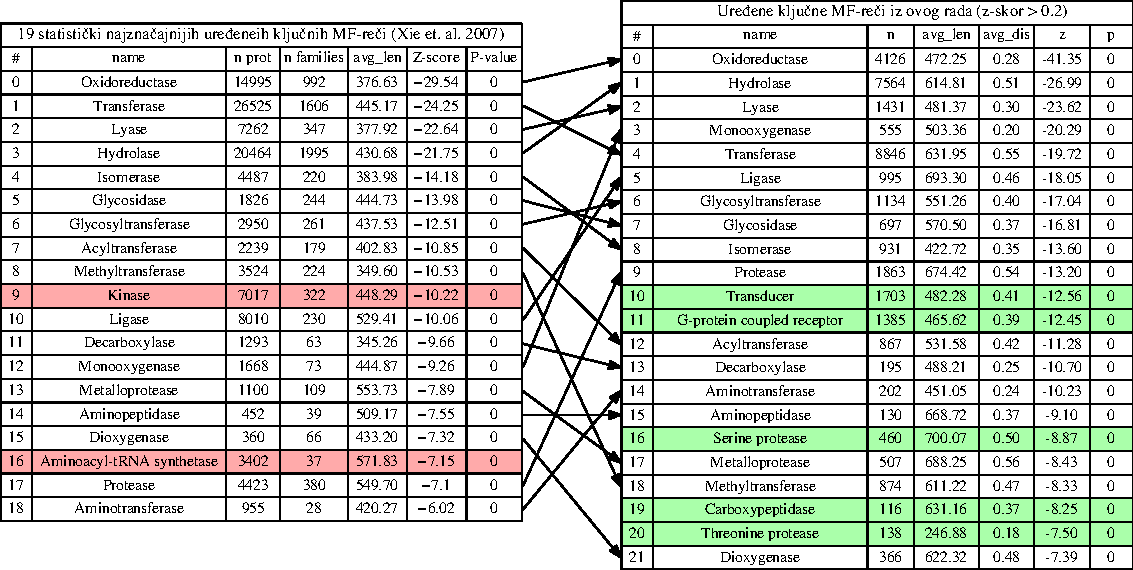
\includegraphics[ scale=0.66]{Figures/plots/order_cmp_a.pdf}
%   \end{figure}
% \end{frame}


\begin{frame}
  \begin{figure}[th]
    \vspace*{-0.8cm}
    \hspace*{-0.45cm}
    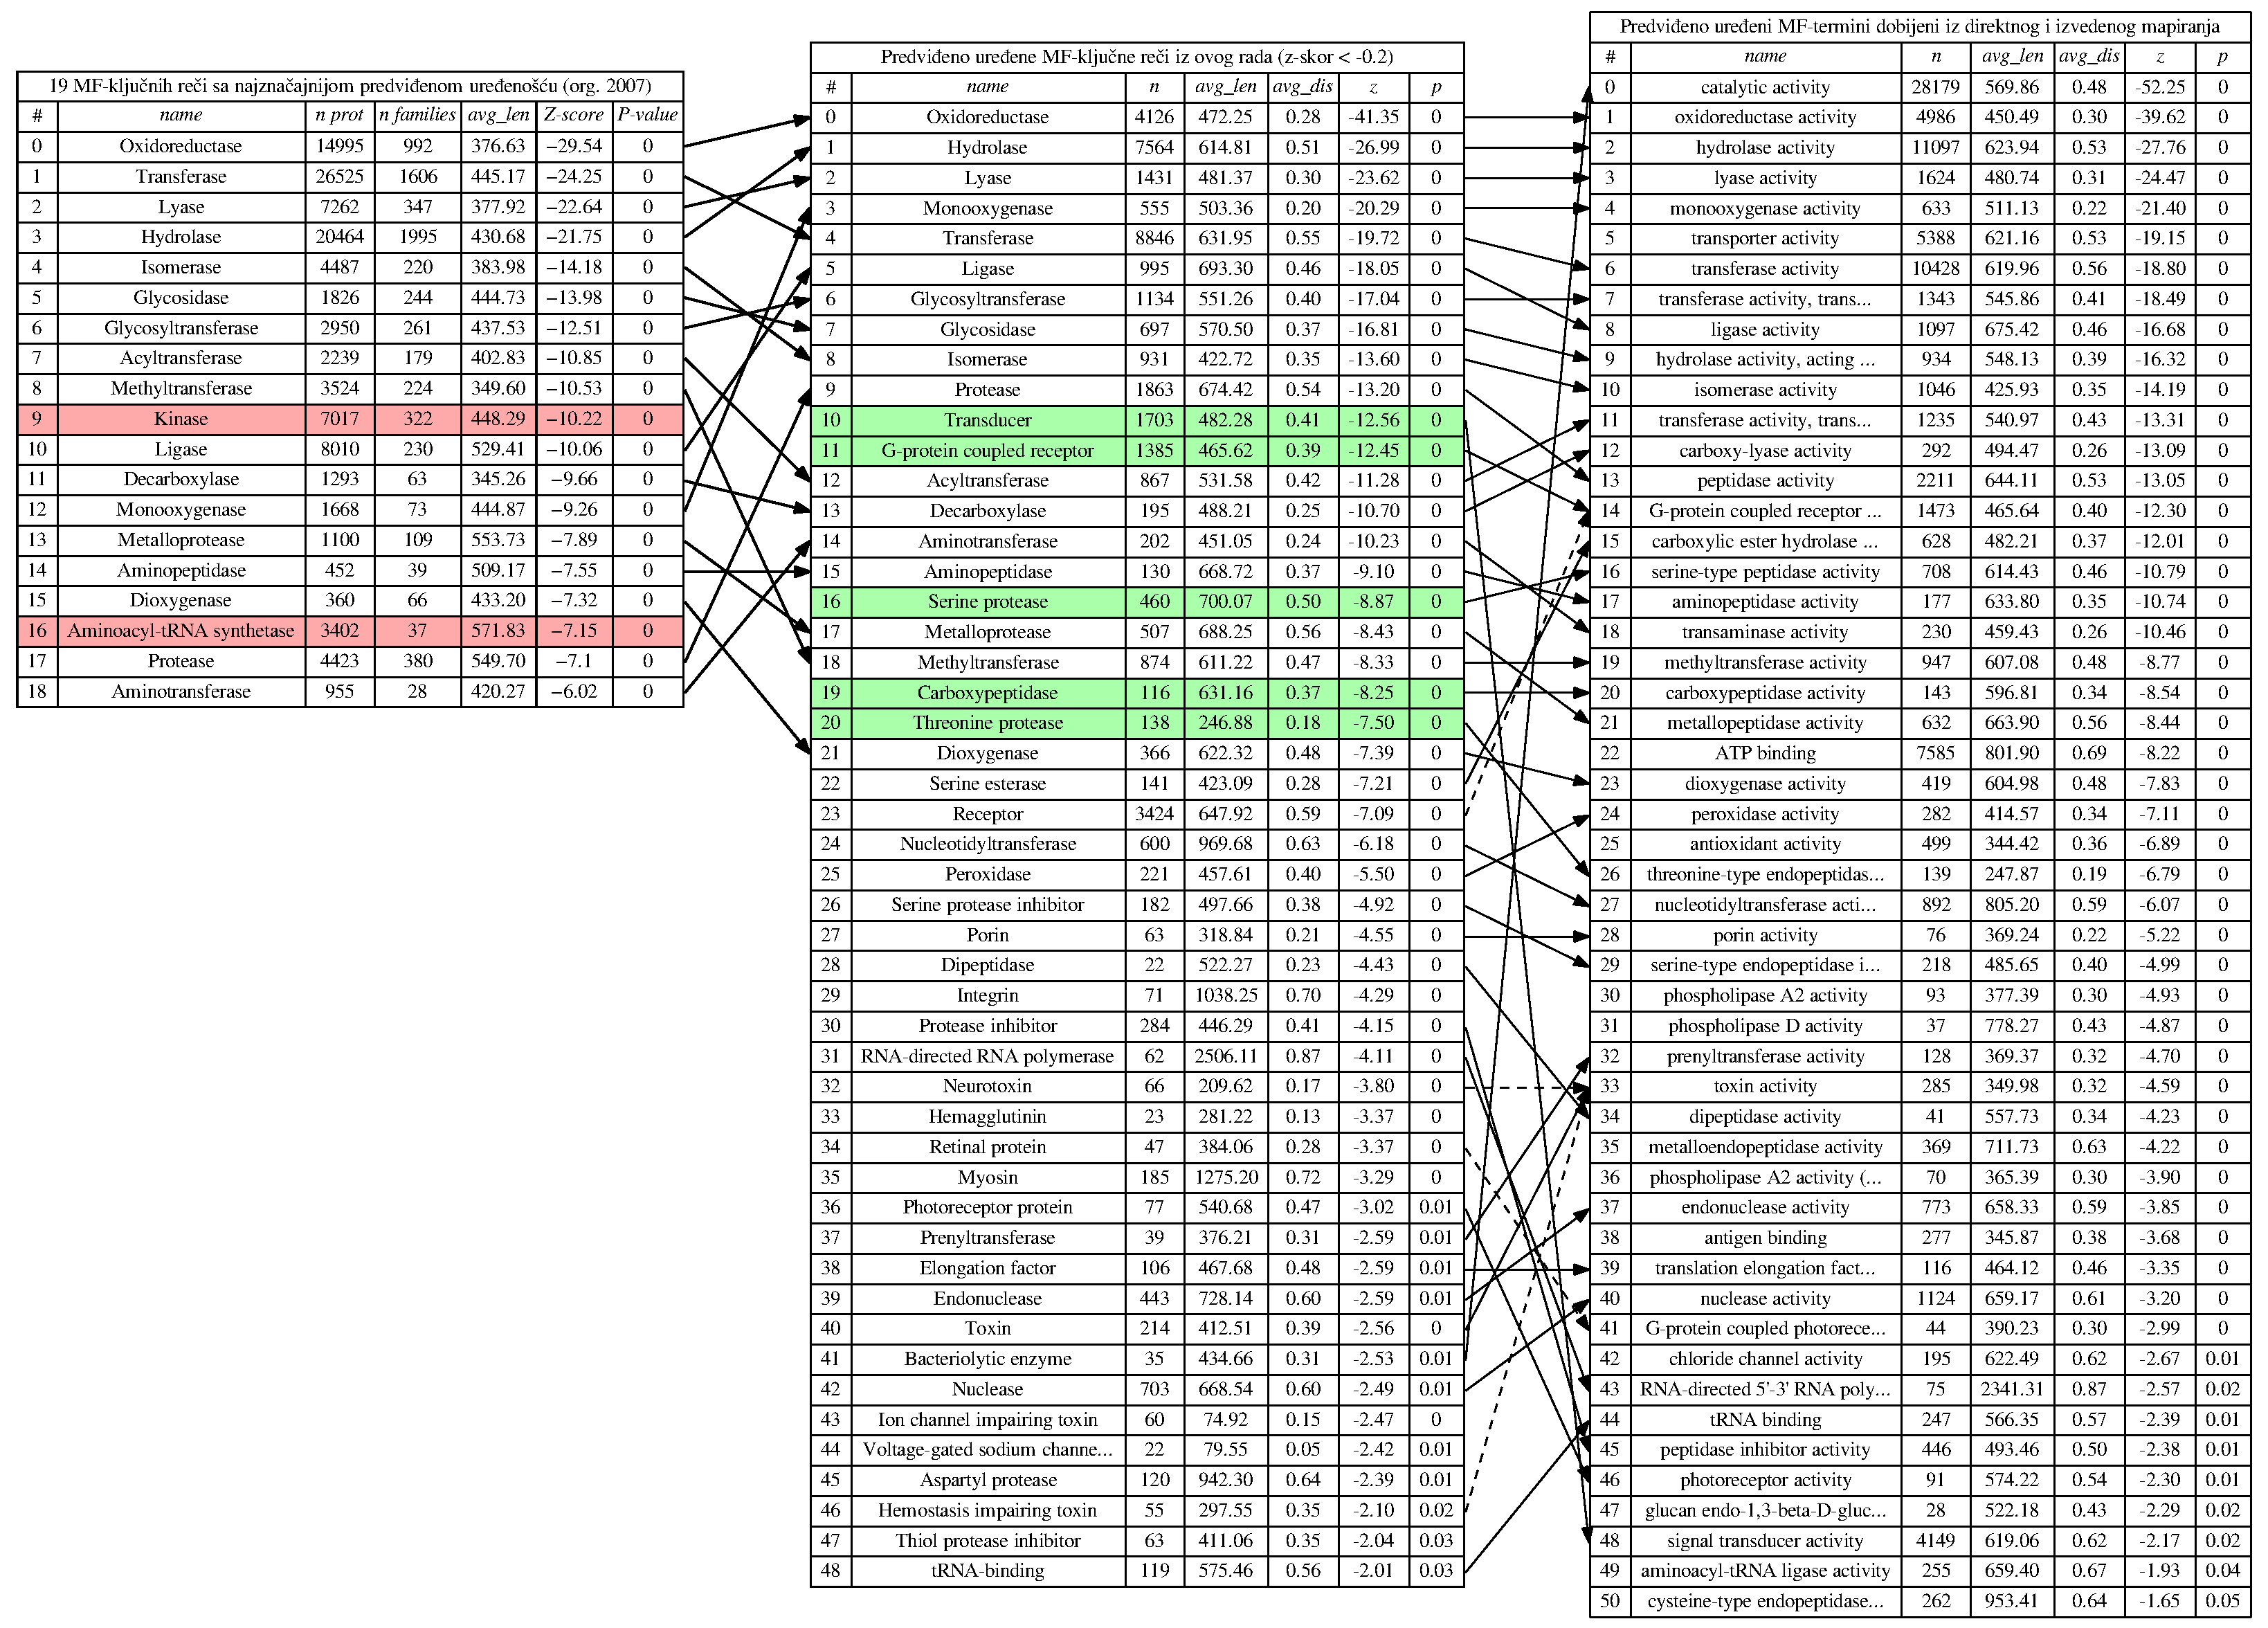
\includegraphics[ scale=0.23]{Figures/plots/order_cmp.pdf}
  \end{figure}
\end{frame}

\begin{frame}
  \begin{figure}[th]
    \vspace*{-0.8cm}
    \hspace*{-0.45cm}
    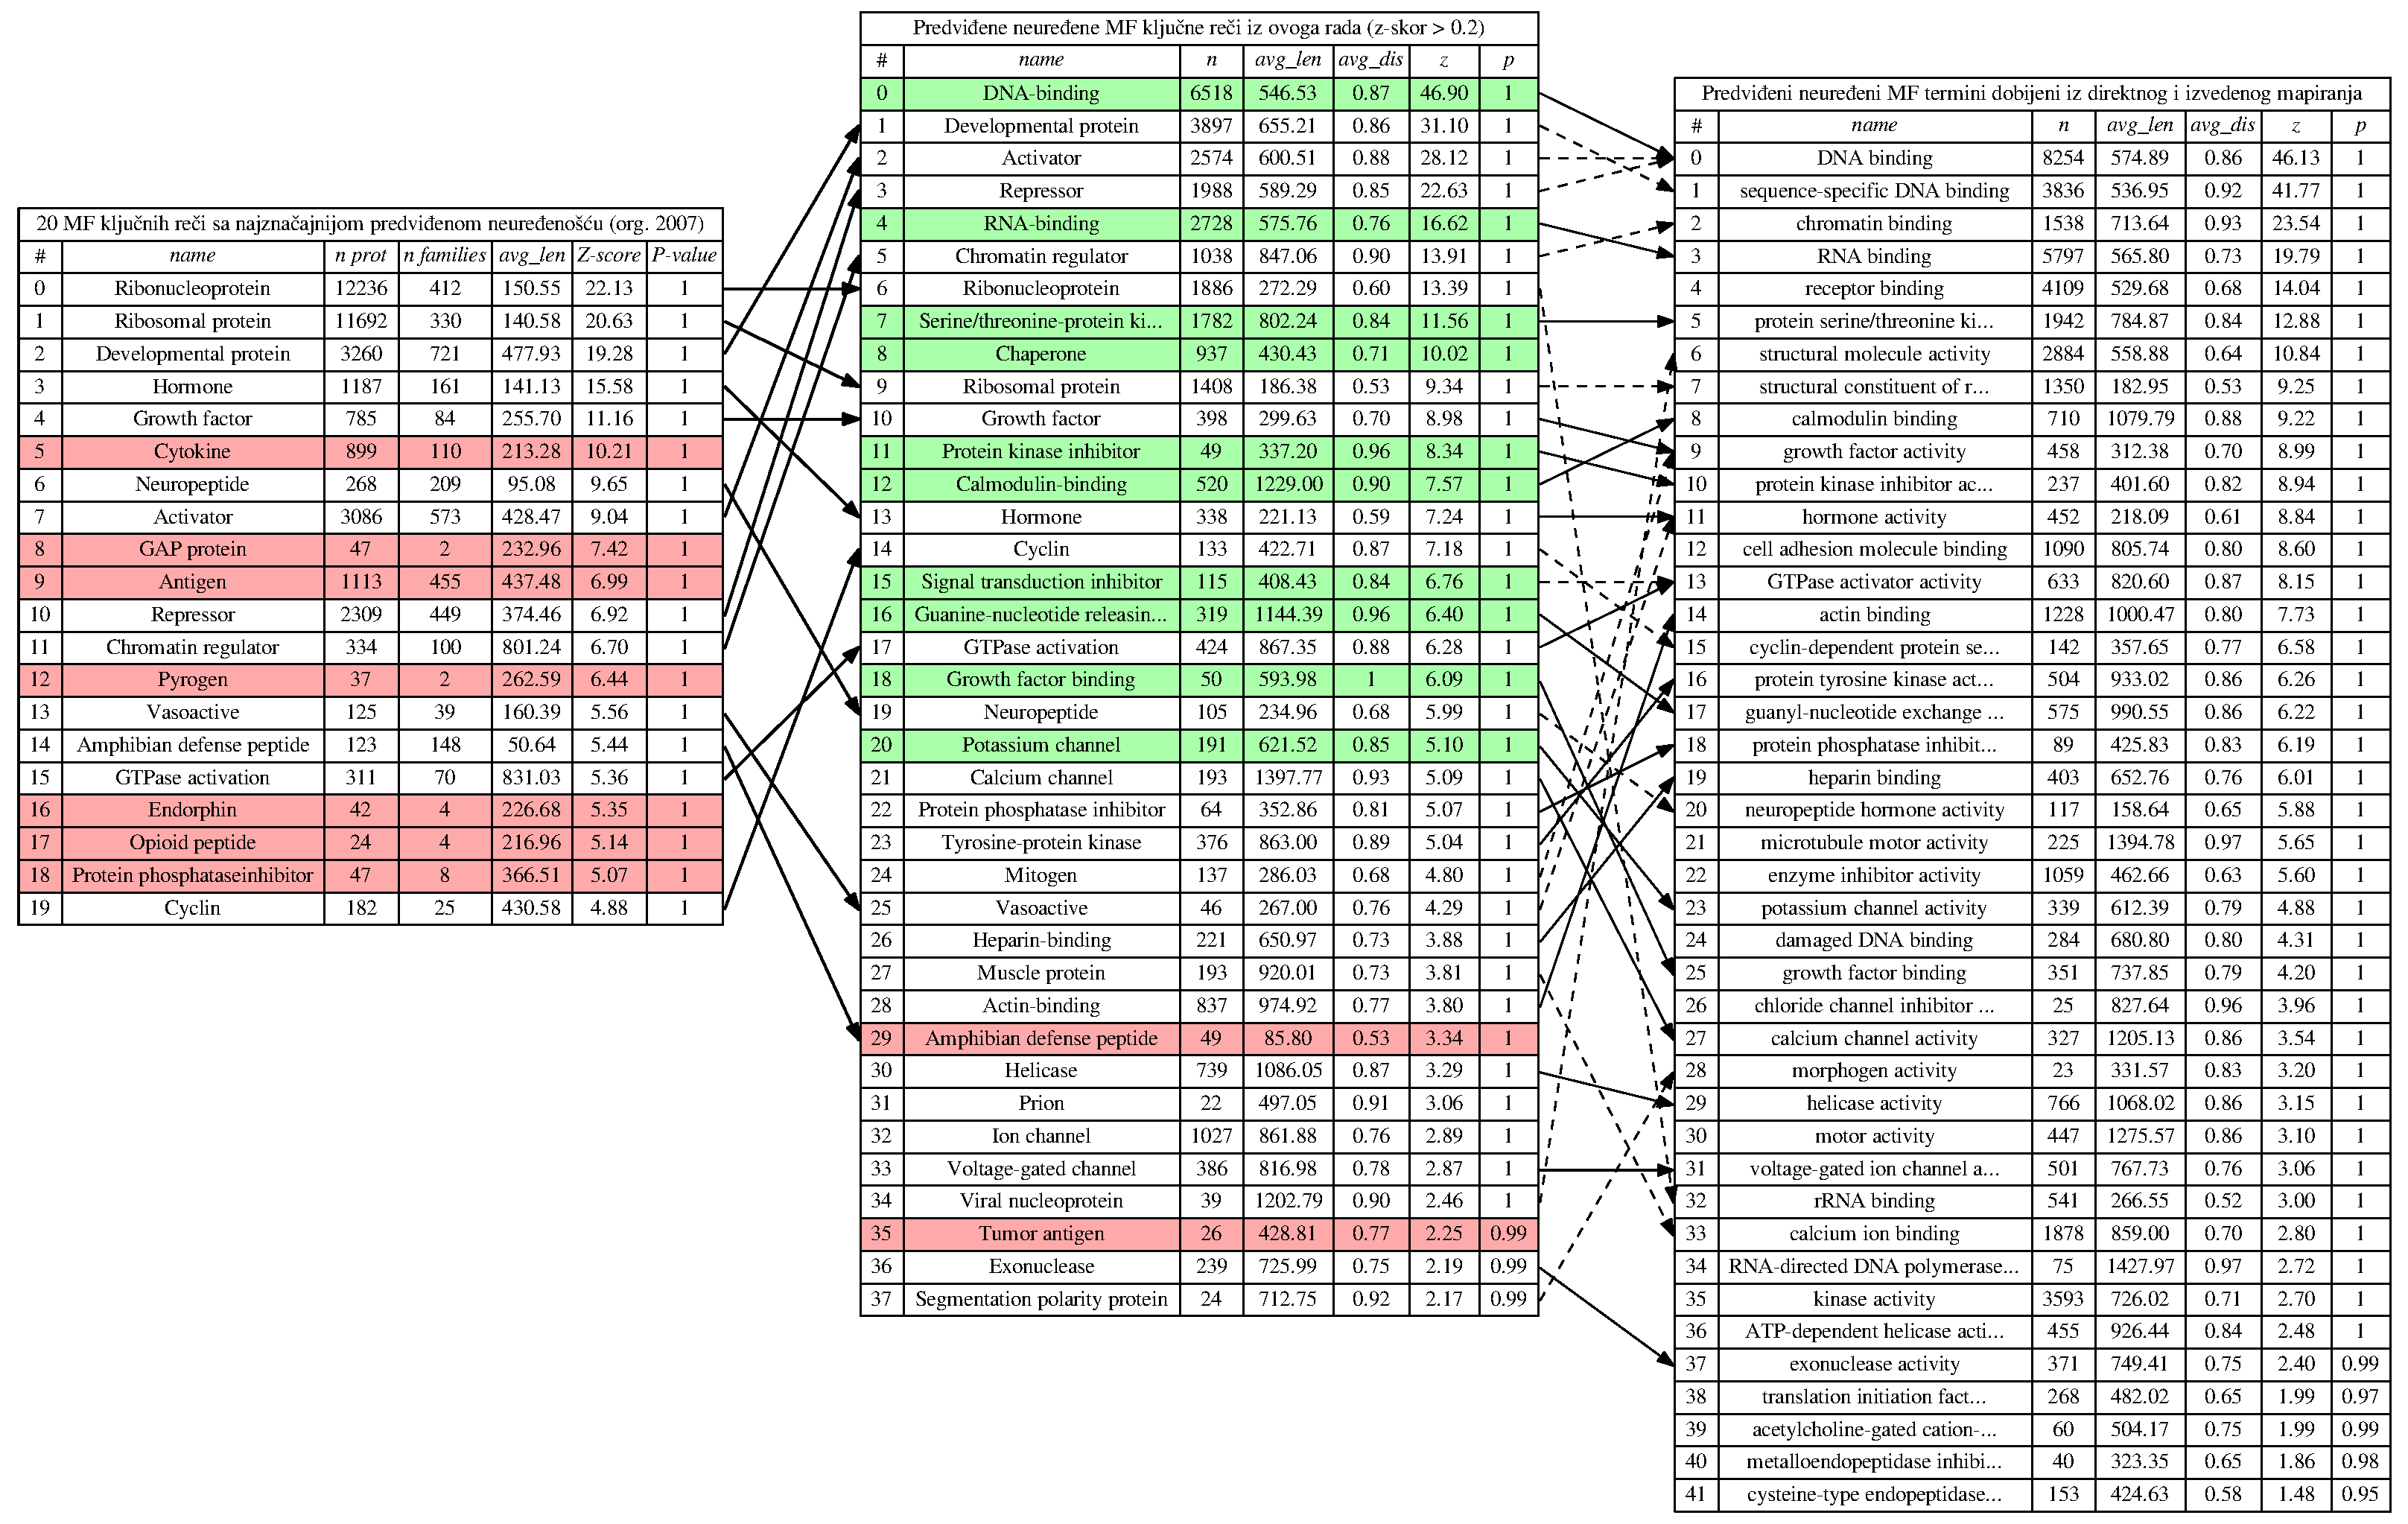
\includegraphics[ scale=0.23]{Figures/plots/disorder_cmp.pdf}
  \end{figure}
\end{frame}


% \begin{frame}
%   \begin{figure}[th]
%     \centering
%     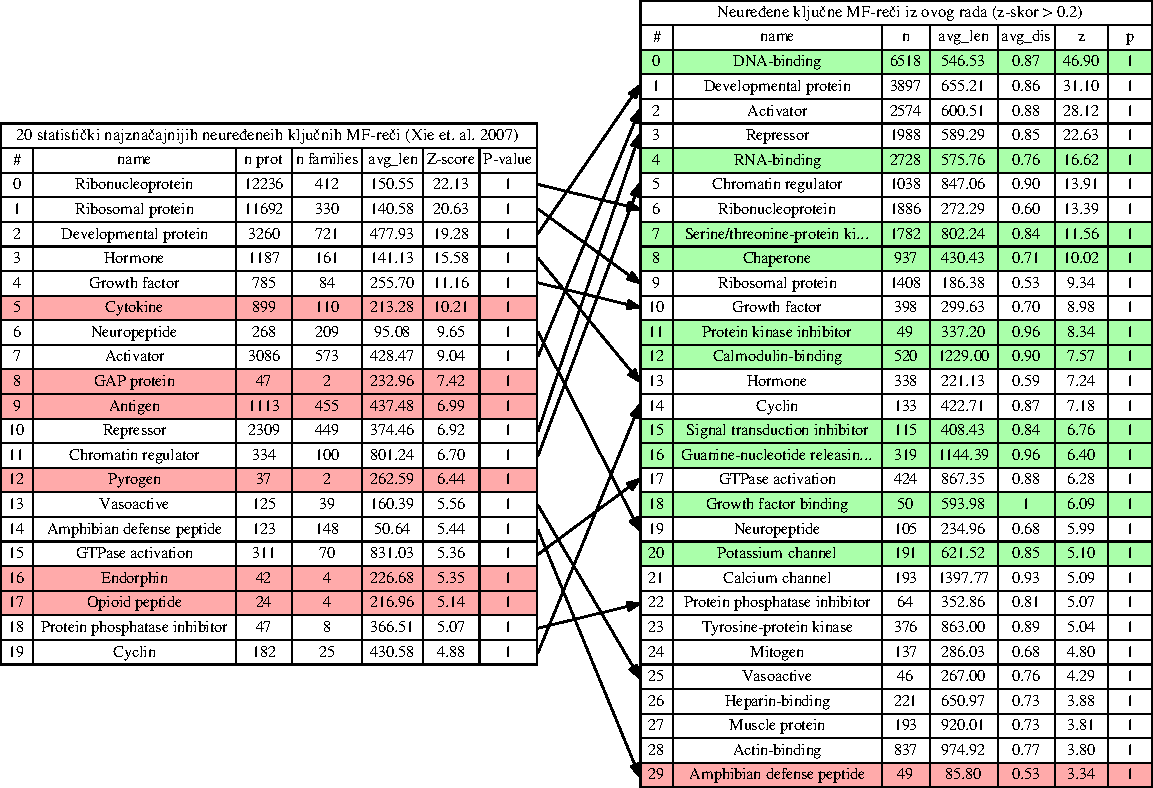
\includegraphics[ scale=0.60]{Figures/plots/disorder_cmp_a.pdf}
%   \end{figure}
% \end{frame}

% \begin{frame}
%   \begin{figure}[th]
%     \vspace{-0.1cm}
%     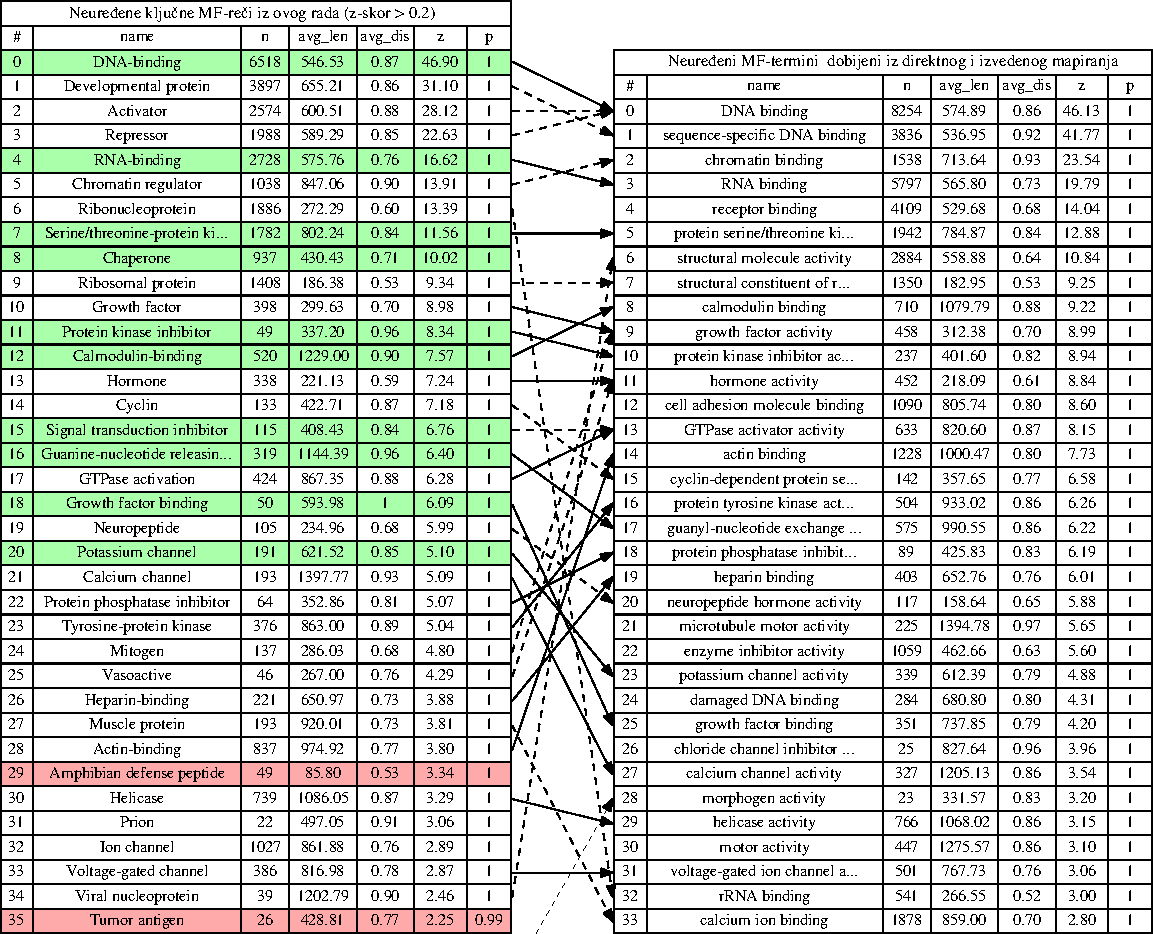
\includegraphics[ scale=0.55]{Figures/plots/disorder_cmp_b.pdf}
%   \end{figure}
% \end{frame}

\subsection{DAG, MF-termini}

\begin{frame}
  \begin{figure}
    \vspace{-0.7cm}
    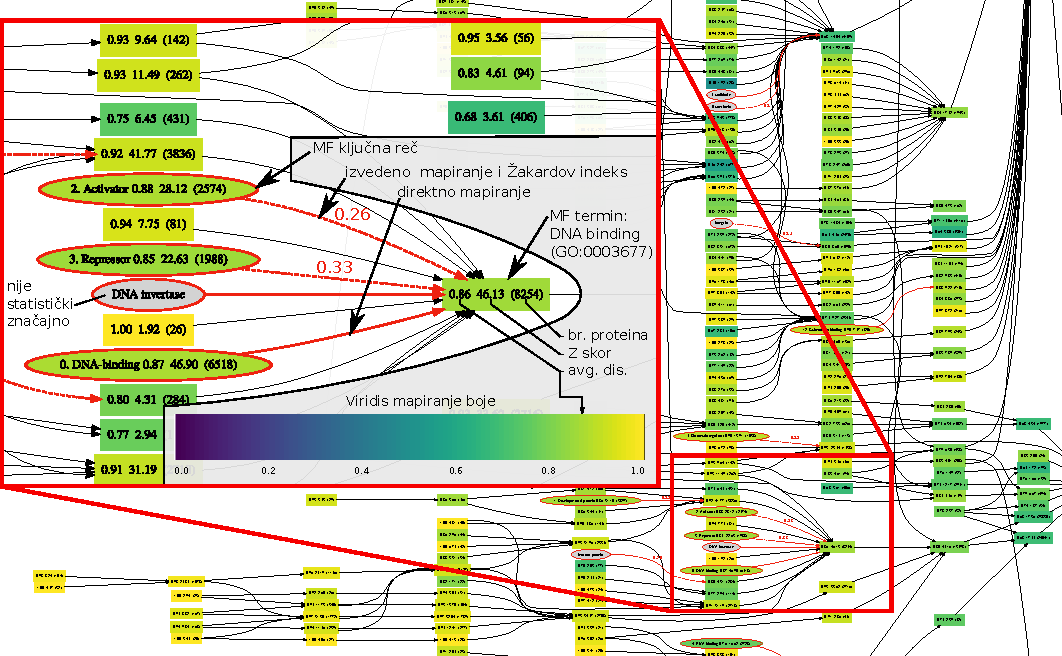
\includegraphics[ scale=0.75]{Figures/plots/disorder_example.pdf}
  \end{figure}
\end{frame}


% \subsection{Odnos prosečne dužine i p}
%
% \begin{frame}
%   \begin{figure}
%     \centering
%     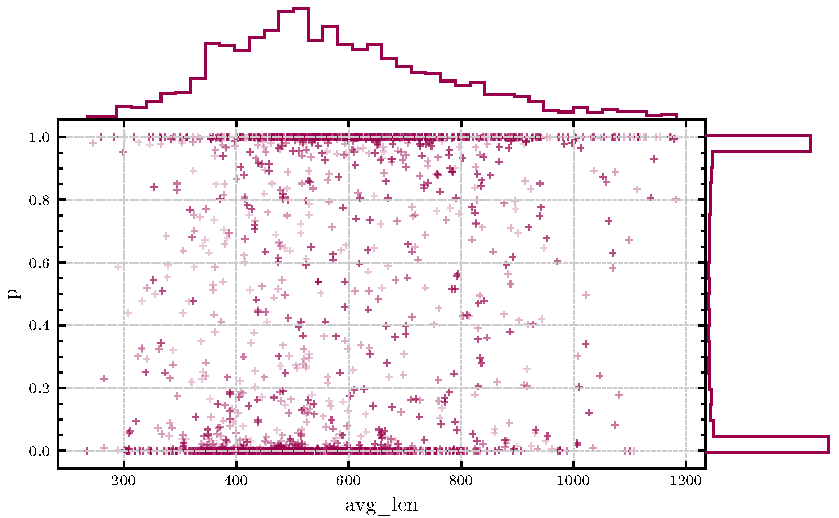
\includegraphics[scale=0.86]{Figures/plots/avg_len2p.pdf}
%   \end{figure}
% \end{frame}


\subsection{Odnos neurđenosti i p}
\begin{frame}
  \begin{figure}
    \centering
    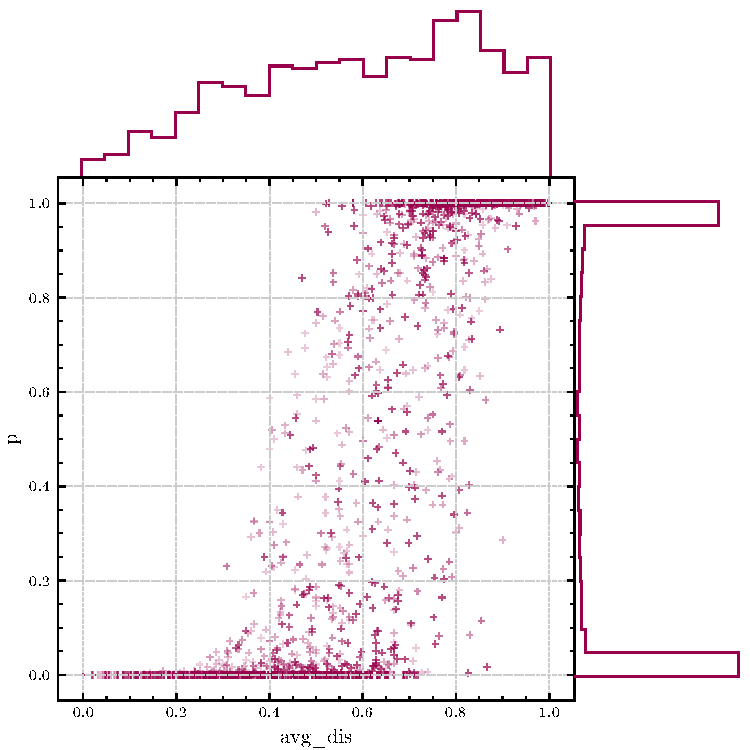
\includegraphics[scale=0.6]{Figures/plots/avg_dis2p.pdf}
  \end{figure}
\end{frame}

\section{Kraj}

\begin{frame}
  \begin{center}
    \Huge Hvala :)
  \end{center}
\end{frame}



\end{document}
